%% ============================================================
%%  Chapter 2 — Proof of Concept: Polymer-Based Composite
%%              Organic Memristive Devices
%%
%%  Author : Carlos David Prado-Socorro
%%  Date   : April 2026
%%  Institution : ICMol, Universitat de València
%%
%%  Compile with: pdflatex → biber → pdflatex × 2
%%  (or use latexmk -pdf -biber)
%% ============================================================

%% ---- Standalone preamble (skipped when \include'd from thesis.tex) ----
%% Chapter-2-specific packages (chemfig) are also loaded by thesis.tex so
%% the chapter compiles in either mode.
\ifdefined\thesismode\else
  \documentclass[12pt, twoside]{report}

  %% Shared thesis formatting (17x24 cm trim, 1.5 line spacing,
  %% two-sided layout, math/chemistry/graphics/bibliography stack).
  %% See chapters/thesis-format.sty for details.
  \usepackage{thesis-format}

  \addbibresource{../bibliography/references.bib}

  \usepackage{chemfig}        % structural formulae; not needed in other chapters

  \begin{document}
  \setcounter{chapter}{1}     % This is Chapter 2 when built standalone
\fi

%% --- Chapter-2-specific macros (safe to (re)declare in document body) ---
\DeclareSIUnit{\rpm}{rpm}     % rpm unit for siunitx (spin-coating speeds)

\newcommand{\SY}{\textit{Super Yellow}}
\newcommand{\HybraneFull}{\textit{Hybrane}\textsuperscript{\textregistered} DEO750 8500} % full grade name; use once at first mention
\newcommand{\Hybrane}{\textit{Hybrane}} % short form for all subsequent mentions
\newcommand{\LiTf}{LiOTf}     % lithium triflate; full name + \ce{LiCF3SO3} given at first use (matches ch.1)
\newcommand{\STM}{short-term memory}
\newcommand{\LTM}{long-term memory}
\newcommand{\STDP}{STDP}      % long form ("spike-timing dependent plasticity") spelled out at first use
\newcommand{\EPSC}{EPSC}      % long form ("excitatory post-synaptic current") spelled out at first use
\newcommand{\ITO}{ITO}        % long form ("indium tin oxide") spelled out at first use
\newcommand{\twoterminal}{two-terminal}
\newcommand{\chTwoSIRef}[1]{\ifdefined\thesismode\cref{#1}\else Appendix~A\fi}

%% ============================================================
\chapter{Proof of Concept: Polymer-Based Composite Organic Memristive Devices}\label{ch:poc}
%% ============================================================

%% ------------------------------------------------------------
\section{Introduction and Motivation}\label{sec:ch2_intro}
%% ------------------------------------------------------------

This chapter reports the proof-of-concept polymer-electrolyte memristive device announced at the end of \cref{ch:intro}. The composite combines a semiconducting poly(phenylene vinylene) (PPV) derivative (\SY{}, SY), an oxygen-rich hyperbranched polyester-amide ion-conducting host (\HybraneFull{}), and a dissociated lithium salt (lithium triflate, \LiTf{}, \ce{LiCF3SO3}), all processed from a common solvent into a standard \twoterminal{} (2-T) sandwich on indium tin oxide (\ITO{}) and silver. The chapter has two purposes within the thesis. First, it tests whether the materials logic of \cref{sec:polymer_electrolyte_composites} translates into a working device that supports the full set of synaptic functions in a single platform. Second, it isolates the mechanistic ingredient (the cation--host coordination chemistry) that the comparative work of \Cref{ch:comparative} then tests across cations and compositions.

At the start of this work the literature already contained several partial demonstrations of these functions in different architectures (reviewed in \cref{subsec:organic_precedents}): ion-mediated analogue switching in multi-layer polyaniline junctions~\cite{Erokhin2005, Smerieri2008, Berzina2009}, bistable ionic redistribution in a light-emitting memristor~\cite{Zakhidov2010}, tunable short-to-long-term transitions in a partially-irreversible redox device~\cite{Liu2016, Heremans2011}, and reversible analogue control in three-terminal organic electrochemical transistors~\cite{Gkoupidenis2015, Xu2016, VanDeBurgt2017, Fuller2019}. Each covered part of the specification developed in \cref{subsec:why_hw} (analogue, reversible, multi-state, low-energy conductance changes set by electrical pulses), but their combination in a single two-terminal organic device with an interpretable ion-mediated mechanism remained, at that point, an open problem.

The active-layer logic adopted here is the composite logic of \cref{subsec:composite_rationale}. The three functional roles --- electronic transport, ionic transport, and mobile-charge supply --- are assigned to three different components, so that each role can be tuned chemically without redesigning the rest of the stack. \SY{} supplies the electronic-conductance pathway. \Hybrane{} supplies an amorphous, low-crystallinity ion-transport host with a high density of hard oxygen donors. \LiTf{} supplies a hard alkali cation paired with a soft, charge-delocalised anion, so that the cation--host and anion--host interactions are asymmetric in the hard--soft acid--base sense of Pearson~\cite{Pearson1963}. The mechanistic account developed in \cref{sec:mechanism} attributes the two memory regimes to this asymmetry.

The chapter shows that the composite supports, in a single 2-T platform, a full set of synaptic functions that fall into two families. The first family comprises three dynamical measurements: current--voltage hysteresis characteristic of memristive switching, potentiation as a function of the number of applied voltage pulses, and depotentiation as a function of the delay before read-out. These three measurements recur, on the same 2-T device geometry, throughout the comparative work of \Cref{ch:comparative,ch:temporal}, and are introduced here as an explicitly named set. The second family comprises extended synaptic protocols that build on the first and are specific to this chapter: excitatory post-synaptic current (\EPSC{}) responses, demonstrated here with four readily distinguishable readout states; the resolution of the depotentiation measurement into a short-lived and a longer-lived memory regime, denoted \STM{} (STM) and \LTM{} (LTM) following the convention of the artificial-synapse literature~\cite{Kim2018,VanDeBurgt2018}; and spike-timing dependent plasticity (\STDP{}) with a time constant in the biologically realistic range~\cite{Bi1998,Kuzum2013}. The interpretation tying these observations together is developed in \cref{sec:mechanism}: the fast component is associated with displacement of the weakly bound triflate anion, while the slow component is associated with displacement of the lithium cation from its hard oxygen coordination environment. The same interpretation yields the cation-substitution prediction tested in \Cref{ch:comparative}.

Within the arc of the thesis the present chapter is narrow in role: it is the only chapter in which the full synaptic suite is treated as the main evidence, while only the three dynamical measurements named above are carried forward to the comparative corpus. The two specific handoffs onto the rest of the thesis are taken up at the end of the chapter.

The chapter proceeds from the materials design and fabrication (\cref{sec:materials_design,sec:device_fab}), through the full electrical characterisation suite (\cref{sec:elec_char}) and its mechanistic interpretation (\cref{sec:mechanism}), to device stability (\cref{sec:stability}), the comparison at the time of publication (\cref{sec:comparison}), and the closing handoff to the comparative and computational work (\cref{sec:ch2_summary}).


%% ------------------------------------------------------------
\section{Materials Design and Composite Formulation}\label{sec:materials_design}
%% ------------------------------------------------------------

\subsection{Design Rationale}\label{subsec:design_rationale}

The operating principle of the device is the same one developed in \cref{subsec:composite_rationale}: ionic migration within a solid-state polymer matrix under an applied electric field redistributes mobile ions near the electrodes, which in turn modifies the energy barriers for charge injection and the doping level of the semiconducting polymer, and therefore the electronic conductance of the device. The composite active layer is built to satisfy three functional requirements simultaneously:

\begin{enumerate}
  \item \textbf{Electronic-conductance pathway:} a semiconducting polymer provides the medium through which the electronic current flows, and whose conductivity is susceptible to modulation by ionic redistribution and electrochemical doping.
  \item \textbf{Ion-transport medium:} a polymer electrolyte provides a structural environment in which dissolved ions remain mobile under an applied field, yet are retarded enough by intermolecular interactions that, once the field is removed, the conductance change persists for seconds --- long enough to be read out --- before fading back toward equilibrium.
  \item \textbf{Ion source:} a dissociated salt provides the mobile charge carriers (a cation and an anion) whose differential response to the field is proposed to underlie the distinct memory regimes reported in \cref{sec:elec_char}.
\end{enumerate}

The composition adopted here is built around a deliberate asymmetry in Lewis acid--base character between the two ions of the salt. \LiTf{} is chosen because \ce{Li+} is a hard Lewis acid with a high charge-to-radius ratio (\(\lambda = z/r \approx\) \SIrange{1.3}{1.7}{\per\angstrom} across the four- to six-fold oxygen coordination that \ce{Li+} adopts in polyether hosts, with \(r_{\mathrm{Li^+}}\) in the range \SIrange{0.59}{0.76}{\angstrom} for the corresponding Shannon effective radii~\cite{Shannon1976}), whereas the triflate anion \ce{CF3SO3-} is a soft Lewis base with a diffuse, low-charge-density anionic centre. The ion-transport polymer, \Hybrane{}, contains a high density of ether and ester oxygen atoms that act as hard Lewis bases. Under the hard--soft acid--base (HSAB) reasoning of Pearson~\cite{Pearson1963} already used in \cref{subsec:ion_conducting_polymers}, hard acids associate preferentially with hard bases. The \ce{Li+} cations are therefore tightly coordinated by the oxygen atoms of \Hybrane{}, while the \ce{CF3SO3-} anions interact only weakly with the host. Under bias, the weakly coordinated triflate anions are displaced at low voltage, while the strongly coordinated lithium cations require a substantially higher field to break free of their coordination environment. This differential mobility is proposed as the molecular origin of the two memory regimes (\STM{} and \LTM{}) reported below.

\subsection{Super Yellow: The Semiconducting Polymer}\label{subsec:sy}

\SY{} (commercial PDY-132, Merck) is the semiconducting PPV-family copolymer in the blend. Its role in the proof-of-concept device is to provide the electronic-conductance path whose injection barriers and local doping state can be modulated by mobile ions. The relevant material facts for the main argument are its solution processability in cyclohexanone, its established use in organic light-emitting devices~\cite{Friend1999}, and frontier levels of approximately \(E_{\mathrm{HOMO}}=\SI{-5.4}{\electronvolt}\) and \(E_{\mathrm{LUMO}}=\SI{-3.0}{\electronvolt}\)~\cite{Zhang2015}. The full copolymer name and component-level notes are collected in \chTwoSIRef{app:ch2_materials_fabrication}.

\subsection{Hybrane DEO750 8500: The Ion-Transport Polymer}\label{subsec:hybrane}

\Hybrane{} is an oxygen-rich hyperbranched polyester-amide~\cite{Froehling2004}. In this chapter it is used as the ion-transport host: ether and ester oxygen atoms provide hard Lewis-base coordination sites for alkali cations, while the hyperbranched architecture suppresses crystallisation and keeps the blend amorphous. Ion motion is therefore treated as segmental-motion-assisted hopping between local coordination environments, in the polymer-electrolyte picture introduced in \cref{subsec:ion_conducting_polymers}. The relevant migration activation scale is of order \SI{50}{\kilo\joule\per\mol} for polymer electrolytes near room temperature~\cite{Gray1991}; the longer discussion of host structure and transport is in \chTwoSIRef{app:ch2_materials_fabrication}.

\subsection{Lithium Triflate: The Ionic Salt}\label{subsec:litf}

\LiTf{} (lithium trifluoromethanesulfonate, \ce{LiCF3SO3}) supplies the mobile ions. It is compatible with the cyclohexanone-processed \SY{}/\Hybrane{} blend and is widely used in polymer-electrolyte and LEC systems~\cite{Pei1995,Wagberg2008}. Mechanistically, its value is the contrast between \ce{Li+}, a small hard Lewis acid, and \ce{CF3SO3-}, a charge-delocalised soft anion. The chapter uses that asymmetry to interpret the two relaxation regimes, while the detailed ion-pairing rationale is kept in \chTwoSIRef{app:ch2_materials_fabrication}.

\subsection{Composite Formulation and Preparation}\label{subsec:formulation}

The active layer uses a mass ratio of \SY{}:\Hybrane{}:\LiTf{} = 1:0.30:0.09, processed from cyclohexanone under dry nitrogen. After mixing, the final solution concentrations are \SI{8.72}{\milli\gram\per\milli\litre} (\SY{}), \SI{2.62}{\milli\gram\per\milli\litre} (\Hybrane{}), and \SI{0.78}{\milli\gram\per\milli\litre} (\LiTf{}). The ratio is the optimised formulation reported in the published proof-of-concept work~\cite{PradoSocorro2022}: higher salt contents degraded film homogeneity, whereas lower salt contents reduced the available mobile-carrier density. Detailed solution preparation and optimisation notes are given in \chTwoSIRef{app:ch2_materials_fabrication}. The same formulation had also been validated in related \SY{}/\Hybrane{}/lithium-salt LECs with long electroluminescent operation~\cite{Mardegan2021}.


%% ------------------------------------------------------------
\section{Device Architecture and Fabrication}\label{sec:device_fab}
%% ------------------------------------------------------------

\subsection{Device Geometry: The Two-Terminal Vertical Structure}\label{subsec:device_geometry}

The device adopts a vertical sandwich geometry, in which the active layer is placed between a bottom transparent electrode and a top metallic electrode (see \cref{fig:device_schematic}). This 2-T architecture is the simplest memristive configuration available: it contains no gate electrode and requires no transistor to address the device, in contrast to the \textit{three-terminal} (3-T) organic synaptic transistors discussed in \cref{subsec:organic_precedents}~\cite{Gkoupidenis2015, Xu2016, Gkoupidenis2017}.

\begin{figure}[htbp]
  \centering
  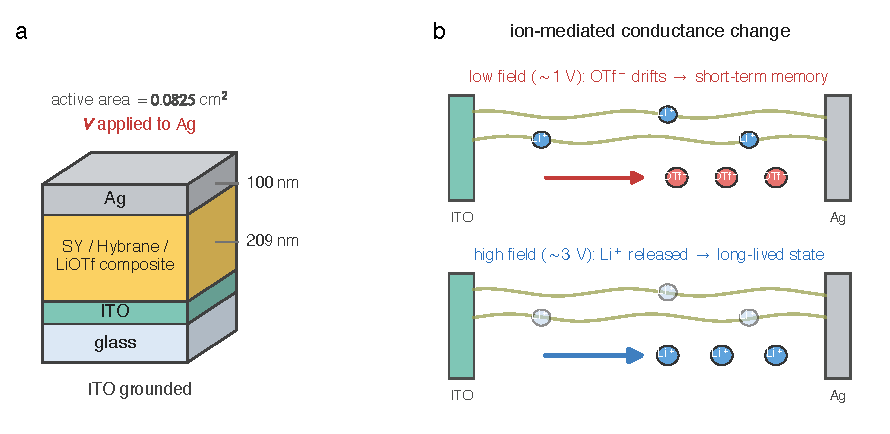
\includegraphics[width=\linewidth]{../figures/chapter2/device_schematic.pdf}
  \caption[Two-terminal device architecture]{Schematic of the two-terminal vertical synaptic device and active-layer mechanism. The device stack is ITO-glass / \SY{}/\Hybrane{}/\LiTf{} composite / Ag; the composite separates the electronic pathway, ion-transport host, and mobile-ion supply. The proposed mechanism assigns the faster STM response to weakly coordinated triflate redistribution and the longer-lived state to displacement of strongly coordinated \ce{Li+}. Schematic generated from the device geometry and mechanism reported in Ref.~\cite{PradoSocorro2022}.}
  \label{fig:device_schematic}
\end{figure}

The 2-T choice matters for two reasons. First, it reduces fabrication complexity, given that the device is made by a sequence of only three depositions (ITO substrate, spin-coated active layer, evaporated metal), which makes the same stack compatible with the comparative corpus of \Cref{ch:comparative}. Second, a 2-T device that shows coexisting \STM{} and \LTM{} without an independent gating signal shows that the memory physics is intrinsic to the active material, rather than being supplied externally by a gate field acting on a separate channel.

The bottom electrode is a pre-patterned layer of \ITO{} deposited on borosilicate glass. ITO combines optical transparency with adequate electronic conductance ($\sigma \approx \SI{e4}{\siemens\per\centi\metre}$)~\cite{Kim1999}, allowing optical inspection of the active layer and characterisation of the device stack by techniques such as UV-Vis spectroscopy and electroluminescence imaging. The work function of ITO ($\Phi_{\mathrm{ITO}} \approx \SI{4.7}{\electronvolt}$) is well matched to the ionisation potential of PPV-family semiconductors~\cite{Ramsdale2002}, facilitating hole injection into the active layer.

The top electrode is silver (Ag), deposited by thermal evaporation. Ag was selected over gold for reasons of cost and practical feasibility; its work function ($\Phi_{\mathrm{Ag}} \approx \SI{4.3}{\electronvolt}$) creates a modest electron injection barrier with the \SY{} conduction band, consistent with asymmetric injection conditions often observed in LEC-type structures~\cite{deMello1998}. The junction active area defined by the shadow mask geometry is \SI{0.0825}{\square\centi\metre}.

\subsection{Fabrication and Active-Layer Morphology}\label{subsec:fabrication_morphology}

ITO-patterned glass substrates were cleaned by sequential ultrasonication, dried under nitrogen, and transferred into a nitrogen glovebox. The composite solution was spin-coated at \SI{2000}{\rpm} for \SI{60}{\second} and annealed at \SI{75}{\celsius} for \SI{3}{\hour}. Contact profilometry gave an active-layer thickness of \SI{209}{\nano\metre} at this spin speed, and tapping-mode AFM showed smooth films with RMS roughness in the range \SIrange{1}{3}{\nano\metre} across the investigated processing window~\cite{PradoSocorro2022}. The spin-speed optimisation, profilometry method, AFM parameters, and supporting morphology evidence are reported in \chTwoSIRef{app:ch2_morphology_stability}.

The top electrode was \SI{100}{\nano\metre} of Ag deposited by thermal evaporation through a shadow mask. The mask defines a junction area of \SI{0.0825}{\square\centi\metre}. Detailed cleaning and evaporation parameters are collected in \chTwoSIRef{app:ch2_materials_fabrication}; the main point for the chapter is that the complete stack is fabricated by solution processing plus one metal evaporation step.


%% ------------------------------------------------------------
\section{Electrical Characterisation}\label{sec:elec_char}
%% ------------------------------------------------------------

Electrical measurements used a Keithley 2450 SourceMeter in a custom probe station. Unless otherwise stated, measurements were made under nitrogen with voltage applied to the Ag top electrode relative to grounded ITO. Protocol-level details are given in \chTwoSIRef{app:ch2_electrical_protocols}.

The characterisation is organised into two groups, following the distinction drawn in \cref{sec:ch2_intro}. \Cref{subsec:iv_hyst,subsec:pulse_potentiation,subsec:stm_ltm} report the three dynamical measurements that are carried forward to the comparative corpus of \Cref{ch:comparative,ch:temporal} --- current--voltage hysteresis, variable-number-of-pulses potentiation, and variable-delay depotentiation. \Cref{subsec:epsc,subsec:stdp} then report the extended synaptic protocols --- the EPSC multi-state readout and spike-timing dependent plasticity --- which are specific to this device and are not propagated to the later chapters. The short- and long-term memory regimes (\STM{}/\LTM{}) are obtained as an interpretation of the variable-delay depotentiation measurement, and are therefore presented together with it in \cref{subsec:stm_ltm}.

\subsection{Current-Voltage Hysteresis}\label{subsec:iv_hyst}

The fundamental electrical fingerprint of a memristive device is a current-voltage ($I$--$V$) hysteresis loop with a characteristic pinched appearance at zero voltage~\cite{Chua1971, Adhikari2013, Chua2014}. This shape arises because, at $V = 0$, the net current is zero regardless of the history of the device (a memristor cannot spontaneously drive current), yet the \textit{slope} of the $I$--$V$ curve at zero voltage (i.e., the instantaneous conductance) depends on the history of applied voltage.

\Cref{fig:iv_hyst} shows the $I$--$V$ curves obtained by applying successive triangular voltage sweeps to the device at a sweep rate of \SI{0.25}{\volt\per\second}, with the voltage ramped from \SI{0}{\volt} to a maximum of \SI{+1.2}{\volt} and back to \SI{0}{\volt} (single polarity, positive). A waiting period of \SI{10}{\second} was observed between successive sweeps to allow partial ionic relaxation. Ten sequential sweeps are shown.

\begin{figure}[htbp]
  \centering
  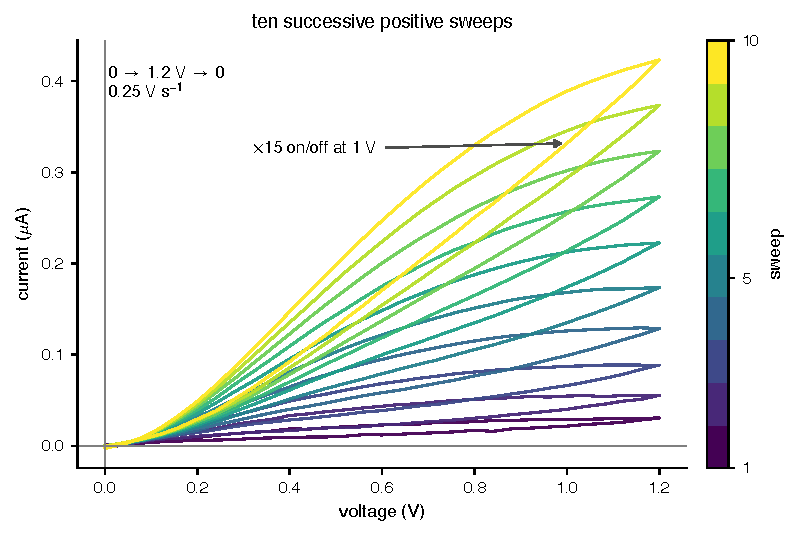
\includegraphics[width=0.86\linewidth]{../figures/chapter2/iv_hyst.pdf}
  \caption[Current--voltage hysteresis]{Current--voltage hysteresis of the composite memristive device. Ten successive positive triangular sweeps (\SIrange{0}{1.2}{\volt}, \SI{0.25}{\volt\per\second}, \SI{10}{\second} between cycles) show a progressive increase of conductance; the current at \SI{1}{\volt} rises by \SI{140}{\percent} from cycle~1 to cycle~2. The clockwise loop closes at the origin (pinched hysteresis) without abrupt switching. Data from Ref.~\cite{PradoSocorro2022}.}
  \label{fig:iv_hyst}
\end{figure}

Several features of these curves are noteworthy:

\paragraph{Progressive increase of conductance.} The current at any fixed voltage \textit{increases} with each successive sweep. From the first to the second cycle, the current at \SI{1}{\volt} increases by \SI{140}{\percent}. By the tenth cycle, the incremental increase from cycle 9 to cycle 10 is \SI{6.3}{\percent} — suggesting that the system is approaching a saturation conductance level asymptotically. This behaviour reflects the progressive redistribution of ions toward the electrodes with each sweep: each successive cycle leaves the ions in a slightly more asymmetric configuration than the previous one, producing a slightly lower resistance state.

\paragraph{Hysteresis without current rectification.} In all cycles, the return sweep (decreasing voltage) produces lower current than the forward sweep (increasing voltage) at the same voltage, generating the characteristic clockwise hysteresis loop for positive voltage sweeps. This is distinct from simple rectification (diode behaviour): a diode would produce the same forward and reverse $I$--$V$ curves; the hysteresis here reflects a time-dependent internal state variable (the ionic configuration) that lags the applied voltage.

\paragraph{Absence of abrupt switching.} Unlike digital resistance switching (SET/RESET transitions), in which the resistance changes abruptly by orders of magnitude at a threshold voltage, the conductance here evolves continuously and smoothly with each cycle. This \textit{analogue} gradation matters for the synaptic role outlined in \cref{subsec:why_hw}, since it allows the device state to be tuned to one of many distinguishable intermediate levels rather than being confined to two (or a few) binary states.

\paragraph{Behaviour under negative polarity.} Application of negative voltage sweeps (not shown individually in the main figure) produces a qualitatively different hysteresis: the current decreases rather than increases with successive negative cycles. This has been attributed to electrochemical side-reactions in the vicinity of the ITO electrode under large negative bias, which generate a thin insulating layer at the ITO/active layer interface analogous to the behaviour reported in MEH-PPV-based LECs~\cite{Wagberg2008, Fang2008}. This effect is not detrimental to memristive operation when devices are used in the single-polarity positive regime.

\subsection{Variable-Number-of-Pulses Potentiation}\label{subsec:pulse_potentiation}

Potentiation by a train of write pulses is the second of the three dynamical measurements introduced at the start of this section. Two complementary experiments are reported: a reversible potentiation/depression cycle that establishes the analogue, multi-state character of the conductance, and a measurement of the conductance change as a function of the number of applied pulses.

\subsubsection{Reversible Potentiation and Depression}

The ability to set the device conductance to a specific value by applying a controlled number of voltage pulses — and to subsequently decrease it back toward the initial value by pulses of opposite polarity — is demonstrated by the potentiation/depression experiment shown in \cref{fig:potentiation}.

A pulsed voltage protocol was applied: 50 consecutive write pulses of \SI{+1}{\volt} amplitude and \SI{0.1}{\second} duration, followed by 50 write pulses of \SI{-2}{\volt}. The conductance was monitored at the peak of each pulse (i.e., at the \SI{+1}{\volt} and \SI{-2}{\volt} levels, respectively). This protocol is analogous to the repeated pre-synaptic stimulation of a biological synapse and its subsequent inhibition.

The results demonstrate that the conductance can be continuously potentiated from its initial value by more than \SI{200}{\percent} during the \SI{+1}{\volt} pulse train, and subsequently depotentiated back toward the initial value during the \SI{-2}{\volt} train. The potentiation and depression curves are smooth and monotonic, without any abrupt transitions. The full reversibility of the process — the conductance returns to a value near the initial level after the complete depression protocol — confirms that the underlying ionic redistribution is non-destructive and does not permanently alter the chemical composition or morphology of the active layer.

The energy cost of each synaptic event (one write pulse of \SI{1}{\volt}, \SI{0.1}{\second}) can be estimated from the average current during the pulse. The resulting energy per event is approximately \SI{50}{\nano\joule}, or approximately \SI{6}{\femto\joule\per\micro\metre\squared} of device area (the \SI{0.0825}{\square\centi\metre} junction). This value is consistent with those reported for organic synaptic devices operating in the picojoule-to-nanojoule range~\cite{Xiao2016}, and comparable to the picojoule-to-nanojoule switching energies reported for inorganic memristive devices~\cite{YangStrukovStewart2013}.

\subsubsection{Quantitative Pulsed Read--Write Protocol}

To quantify the potentiation as a function of pulse number, and to separate the act of writing from the act of reading, a non-perturbing read protocol was adopted; the same protocol is reused for the depotentiation measurement of \cref{subsec:stm_ltm}. The read--write--wait sequence, detailed in \chTwoSIRef{app:ch2_read_write_wait}, comprises three steps:
\begin{enumerate}
  \item \textbf{Read.} A reading pulse ($V_{\mathrm{read}} = \SI{0.5}{\volt}$) is applied to establish the initial conductance $G_0$. This reading voltage is intentionally low: the activation threshold for ionic redistribution in this system was determined by independent experiments to lie above \SI{0.7}{\volt}~\cite{PradoSocorro2022}, so $V_{\mathrm{read}} = \SI{0.5}{\volt}$ measures the conductance state without perturbing it.
  \item \textbf{Write.} A train of $N_{\mathrm{pulses}}$ write pulses ($V_{\mathrm{write}}$, duration \SI{0.1}{\second} each) is applied.
  \item \textbf{Wait and read.} After a waiting time $t_{\mathrm{wait}}$ under open-circuit (high-impedance) conditions, a second reading pulse is applied to measure the final conductance $G_f$.
\end{enumerate}
The conductance change is reported as the percentage ratio $\Delta G = (G_f/G_0) \times 100$.

Between experiments, the device is fully reset by connecting the junction to a short circuit for \SI{300}{\second}, which discharges the ionic double layers and restores the homogeneous equilibrium ion distribution. The suitability of this reset protocol was verified by confirming that $G_0$ returns to its original value within the measurement uncertainty before each new experiment.

\subsubsection{Potentiation as a Function of Pulse Number}

\Cref{fig:npulse} shows the dependence of $\Delta G$ on $N_{\mathrm{pulses}}$ for $V_{\mathrm{write}} = \SI{1}{\volt}$ and $t_{\mathrm{wait}} = \SI{150}{\milli\second}$. The conductance ratio increases monotonically with $N_{\mathrm{pulses}}$, reaching values in excess of $10^3$\% for $N_{\mathrm{pulses}} > 10^3$. The relationship is approximately linear in log-log space for $N_{\mathrm{pulses}} < 100$ and saturates at large pulse numbers, consistent with a scenario in which the degree of ionic asymmetry that can be built up under a given write voltage is bounded by the total number of mobile ionic carriers.

\begin{figure}[htbp]
  \centering
  \begin{subfigure}[t]{0.48\linewidth}
    \centering
    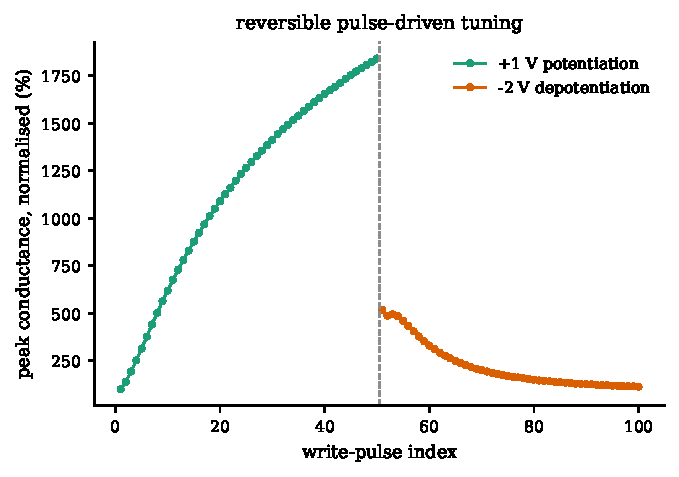
\includegraphics[width=\linewidth]{../figures/chapter2/potentiation_depression.pdf}
    \caption{Reversible potentiation/depression.}
    \label{fig:potentiation}
  \end{subfigure}\hfill
  \begin{subfigure}[t]{0.48\linewidth}
    \centering
    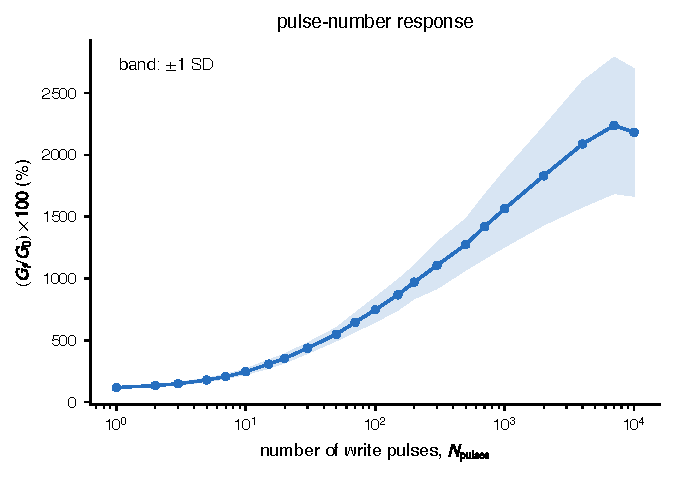
\includegraphics[width=\linewidth]{../figures/chapter2/pulse_number.pdf}
    \caption{Pulse-number response.}
    \label{fig:npulse}
  \end{subfigure}
  \caption[Pulse-driven conductance integration]{Pulse-driven conductance integration in the composite memristive device. \textbf{(a)} Fifty consecutive \SI{+1}{\volt} write pulses continuously potentiate the conductance; subsequent \SI{-2}{\volt} pulses depotentiate it toward the initial state. \textbf{(b)} Dependence of the conductance ratio \((G_f/G_0)\times100\%\) on the number of write pulses for \(V_{\mathrm{write}}=\SI{1}{\volt}\) and \(t_{\mathrm{wait}}=\SI{150}{\milli\second}\). The shaded band is one standard deviation across five independent crossbar pixels on the NM\_v055 substrate. Data regenerated from the local archive associated with Ref.~\cite{PradoSocorro2022}.}
  \label{fig:pulse_integration}
\end{figure}

Within this archived pulse-train dataset, the low-pulse-count response is reproducible to approximately the \SI{10}{\percent} level: for the five independent pixels in \cref{fig:npulse}, the median relative standard deviation is \SI{8.9}{\percent} and the largest value is \SI{11.8}{\percent} over the points with $N_{\mathrm{pulses}} < 100$. The dispersion increases modestly at large pulse numbers, reflecting the probabilistic nature of the ionic migration dynamics at large driving forces.

\subsection{Variable-Delay Depotentiation: Short- and Long-Term Retention}\label{subsec:stm_ltm}

The third dynamical measurement carried through the thesis probes how a written conductance state fades once the drive is removed: the depotentiation of the device measured as a function of the delay before read-out. This is one of the most important characterisation protocols for neuromorphic devices, because it determines whether the device can emulate short-lived and longer-lived synaptic states on experimentally accessible timescales. In the artificial-synapse literature these regimes are commonly labelled \STM{} and \LTM{}; in the present system, the longer-lived regime remains on the sub-minute scale and should therefore be understood operationally rather than as a claim of indefinitely persistent storage.

The measurement reuses the pulsed read--write protocol of \cref{subsec:pulse_potentiation}, with the waiting time $t_{\mathrm{wait}}$ now the swept variable and the pulse number held fixed. \Cref{fig:retention} shows the dependence of $\Delta G$ on $t_{\mathrm{wait}}$ for three excitation conditions: (i) $V_{\mathrm{write}} = \SI{1}{\volt}$, $N_{\mathrm{pulses}} = 10$ (STM, blue); (ii) $V_{\mathrm{write}} = \SI{1}{\volt}$, $N_{\mathrm{pulses}} = 50$ (STM, red); and (iii) $V_{\mathrm{write}} = \SI{3}{\volt}$, $N_{\mathrm{pulses}} = 10$ (LTM, black).

\begin{figure}[htbp]
  \centering
  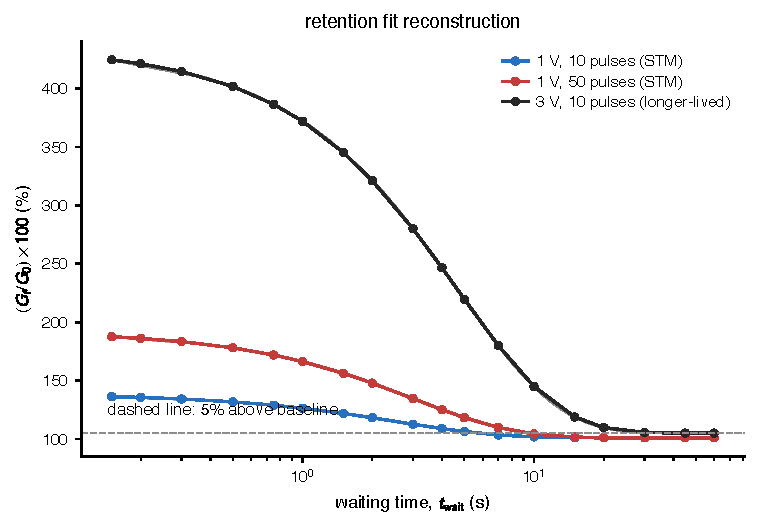
\includegraphics[width=0.82\linewidth]{../figures/chapter2/retention.pdf}
  \caption[Memory retention kinetics]{Memory retention kinetics. Conductance ratio $(G_f/G_0)\times 100\%$ versus waiting time $t_{\mathrm{wait}}$ for STM conditions (\SI{1}{\volt}; 10 and 50 pulses, blue/red) and the longer-lived regime denoted LTM (\SI{3}{\volt}, 10 pulses, black). Solid lines are standard-exponential reconstructions of the form in \cref{eq:retention_exp}; the fit parameters are summarised in \chTwoSIRef{app:ch2_retention_fits}. Data and fit parameters from Ref.~\cite{PradoSocorro2022}.}
  \label{fig:retention}
\end{figure}

For short waiting times ($t_{\mathrm{wait}} < \SI{500}{\milli\second}$ for STM conditions, $t_{\mathrm{wait}} < \SI{2}{\second}$ for LTM conditions), the conductance first \textit{increases} slightly relative to the value immediately after the write pulse train. This counterintuitive behaviour is \emph{not} ascribed to ionic inertia: ion transport in the polymer matrix is strongly overdamped, so any momentum imparted by the field relaxes on a timescale orders of magnitude shorter than the observed enhancement. It is instead attributed to the continued redistribution of ions after the drive is removed. At the end of the pulse train the ionic configuration and its self-consistent space-charge field have not yet reached their quasi-steady profile; the residual internal field, together with the slow advance of the electrochemically doped region near the electrode, continues to raise the conductance for a brief interval before the diffusion-driven relaxation sets in. An analogous transient enhancement following a stimulus train has been described as ``post-tetanic potentiation'' in biological synaptic preparations~\cite{Zucker1989, ZuckerRegehr2002}.

For longer waiting times, the expected exponential relaxation of conductance is observed as the ionic configuration relaxes back toward equilibrium by thermal diffusion. The fit record summarised in \chTwoSIRef{app:ch2_retention_fits} reports least-squares fits in IGOR Pro 8 to a standard exponential:

\begin{equation}
  \frac{G_f(t_{\mathrm{wait}})}{G_0} = R_\infty + A \exp\!\left(-\frac{t_{\mathrm{wait}}}{\tau}\right)
  \label{eq:retention_exp}
\end{equation}

where $\tau$ is the characteristic relaxation time, $A$ is the decaying amplitude, and $R_\infty$ is the long-waiting-time conductance ratio. In other words, the published proof-of-concept fit corresponds to a stretched-exponential model with the stretch exponent fixed at $\beta=1$. No free $\beta$ parameter, confidence interval, or goodness-of-fit statistic was reported for these three traces, so the \cref{ch:poc} evidence is used here only to establish the two experimentally resolved relaxation times, not to claim a fitted distribution of relaxation barriers. The later comparative analysis in \cref{ch:comparative} uses a free-exponent Kohlrausch descriptor only where the DELAYTIME archive is refitted consistently across the comparative corpus.

The fitted characteristic times are $\tau_S = \SI{2.57}{\second}$ for the \SI{1}{\volt}, 10-pulse STM trace, $\tau_S = \SI{3.01}{\second}$ for the \SI{1}{\volt}, 50-pulse STM trace, and $\tau_L = \SI{4.73}{\second}$ for the \SI{3}{\volt}, 10-pulse LTM trace. The corresponding offsets and amplitudes are tabulated in \chTwoSIRef{app:ch2_retention_fits}. The retention time --- defined operationally as the waiting time at which $G_f/G_0$ returns to within \SI{5}{\percent} of the baseline (i.e., $G_f/G_0 < 1.05$) --- is \SIrange{10}{15}{\second} for STM and exceeds \SI{45}{\second} for the longer-lived regime labelled LTM. These values are directly relevant to the timescales of spike-based computation: the \SIrange{10}{15}{\second} STM window is sufficient to maintain working memory over a series of sequential spike inputs, while the $> \SI{45}{\second}$ LTM window shows that the device can preserve a write history over many subsequent events without approaching the retention regime of a conventional non-volatile memory.

The molecular mechanism underlying the STM/LTM distinction is discussed in detail in \cref{sec:mechanism}.

\subsection{Excitatory Post-Synaptic Current}\label{subsec:epsc}

The \EPSC{} measurement is a standard protocol in the field of artificial synaptic devices, designed to quantify the number and stability of distinguishable conductance states accessible to the device~\cite{Kim2018, VanDeBurgt2018}. The protocol employed here closely mimics the biological experiment in which a patch-clamped neuron is subjected to a defined sequence of pre-synaptic inputs and the post-synaptic current is monitored.

The measurement protocol is as follows (\cref{fig:epsc}):
\begin{enumerate}
  \item \textbf{Initialisation.} The device is initialised to its ground state $S_0$ by applying a fixed read-out bias $V_0 = \SI{+1}{\volt}$ for \SI{1}{\second}. This bias differs in purpose from the sub-threshold probe ($V_{\mathrm{read}} = \SI{0.5}{\volt}$) used for the non-perturbing read-out of \cref{subsec:pulse_potentiation,subsec:stm_ltm}: the EPSC states are defined operationally by the current response at a single common read-out bias against which all states $S_0$--$S_4$ are referenced, not by a passive probe required to leave the state untouched.
  \item \textbf{Excitation.} A short positive write pulse of \SI{+2}{\volt} for \SI{50}{\milli\second} is applied; the device is subsequently held at \SI{+1}{\volt} for \SI{1}{\second}, during which the conductance spontaneously relaxes to a new excited steady state $S_1$. The same sequence is repeated to produce a second excited state $S_2$.
  \item \textbf{Inhibition.} Two negative write pulses of \SI{-2.5}{\volt} for \SI{50}{\milli\second} are applied, producing inhibitory states $S_3$ and $S_4$.
\end{enumerate}

The four excited states are readily distinguishable from each other and from the ground state. Defining the \EPSC{} readout ratio $R_n = I_{S_n}/I_{S_0}$ as the signed current response of state $S_n$ normalised to that of the ground state $S_0$ under the fixed read-out bias used in the experiment, the values obtained are: $R_1 = 7.33$, $R_2 = 15.55$, $R_3 = -3.72$, $R_4 = -16.97$. (The ratio is formed from signed currents rather than conductances, so the inhibitory states carry a negative sign; conductance itself remains non-negative throughout.) The large absolute ratios (up to $\sim$16-fold increase or $\sim$17-fold decrease relative to $S_0$) provide a wide margin for reliable state identification in a practical device, even in the presence of noise. The four-state sequence used here is a representative demonstration rather than an upper bound: given the continuous, analogue conductance tunability established in \cref{subsec:pulse_potentiation}, the number of distinguishable readout states is not intrinsically limited to four, and many more intermediate levels could in principle be resolved by the same protocol within the available margin.

The states \(S_1\) and \(S_2\) are reached by \textit{excitatory} (positive polarity) stimulation, while \(S_3\) and \(S_4\) are reached by \textit{inhibitory} (negative polarity) stimulation, in direct analogy with long-term potentiation (LTP) and long-term depression (LTD) at biological synapses. The coexistence of both excitatory and inhibitory states in the same 2-T device, without an independent gate terminal, distinguishes the present platform from the 3-T organic implementations discussed in \cref{subsec:organic_precedents}.

\subsection{Spike-Timing Dependent Plasticity}\label{subsec:stdp}

Spike-timing dependent plasticity is a timing-dependent Hebbian learning rule: it instantiates Hebb's local correlation principle~\cite{Hebb1949} in a form that was later observed experimentally in biological preparations~\cite{Markram1997, Bi1998}. Here the timing delay is defined as \(\Delta t = t_{\mathrm{post}} - t_{\mathrm{pre}}\). With this convention, if the presynaptic neuron fires shortly \textit{before} the postsynaptic neuron (causal ordering, $\Delta t < 0$), the synapse is potentiated (LTP); if the presynaptic neuron fires shortly \textit{after} the postsynaptic neuron (anti-causal ordering, $\Delta t > 0$), the synapse is depressed (LTD). The magnitude of the change decays exponentially with $|\Delta t|$. This temporal asymmetry is essential for the synaptic encoding of causal relationships in neural circuits and underlies the ability of STDP-based learning rules to implement unsupervised feature extraction and pattern recognition~\cite{Bichler2012}.

\subsubsection{Experimental Protocol}

The STDP experiment requires the emulation of pre- and postsynaptic spike waveforms by voltage pulses applied at the two electrodes of the device. In a 2-T device, both pulses must be applied at the same physical terminal (the Ag electrode), so the experimentally measured total voltage $V(t)$ is the algebraic sum of the presynaptic and postsynaptic voltage waveforms separated by the delay $\Delta t$:

\begin{equation}
  V(t) = V_{\mathrm{pre}}(t) + V_{\mathrm{post}}(t + \Delta t)
  \label{eq:stdp_voltage}
\end{equation}

Each spike waveform consists of a unipolar triangular pulse with maximum amplitude $V_{sp}$ and duration \SI{1.2}{\second}. The delay $\Delta t$ was varied from \SI{-600}{\milli\second} to \SI{+600}{\milli\second}. The amplitude $V_{sp} = \SI{1.55}{\volt}$ was chosen to be large enough to activate ionic migration (above the threshold of approximately \SI{0.7}{\volt}) while remaining below the onset of electrochemical degradation of the active layer (conservatively estimated at \SI{2}{\volt} for the pristine device).

For \(\Delta t < 0\) (pre fires before post), the two spike waveforms partially overlap in time with additive polarity, producing a composite pulse whose peak voltage exceeds \(V_{sp}\) and which is directed in the positive sense. The ions then redistribute toward the ITO electrode, the conductance increases, and the device records a net synaptic potentiation.

For \(\Delta t > 0\) (post fires before pre), the overlap produces an anti-causal summation. Depending on the exact waveforms, the effective net voltage can be of reduced amplitude or of reversed polarity relative to the causal case, so the ionic redistribution is either weaker or reversed and the conductance decreases, in the form of a net synaptic depression.

\subsubsection{STDP Curve and Fitting}

\Cref{fig:stdp} shows the measured STDP function: the percentage conductance change $\Delta G$ plotted against the timing delay $\Delta t$. Under the sign convention above, the measured kernel is asymmetric Hebbian: negative $\Delta t$ (causal) produces positive $\Delta G$ (potentiation), and positive $\Delta t$ (anti-causal) produces negative $\Delta G$ (depression). Each branch (potentiation for $\Delta t < 0$, depression for $\Delta t > 0$) is fitted separately, as a function of the absolute delay $|\Delta t|$, by a decaying exponential:

\begin{equation}
  \Delta G(\Delta t) = A_{\pm}\,\exp\!\left(-\frac{|\Delta t|}{\tau_{\pm}}\right) + G_0
  \label{eq:stdp_fit}
\end{equation}

where $A_{\pm}$ and $\tau_{\pm}$ are the branch-specific amplitude and time constant ($+$ for the potentiation branch, $-$ for the depression branch) and $G_0$ is a constant offset. The best-fit values of $\tau_{\pm}$ for both the potentiation and depression branches lie in the range \SIrange{85}{90}{\milli\second}. This is in close quantitative agreement with the characteristic timescale of biological STDP, which is approximately \SI{100}{\milli\second}~\cite{Kuzum2013, Bi1998}. The device, therefore, not only qualitatively replicates the STDP function but does so with biologically realistic time constants.

\begin{figure}[htbp]
  \centering
  \begin{subfigure}[t]{0.48\linewidth}
    \centering
    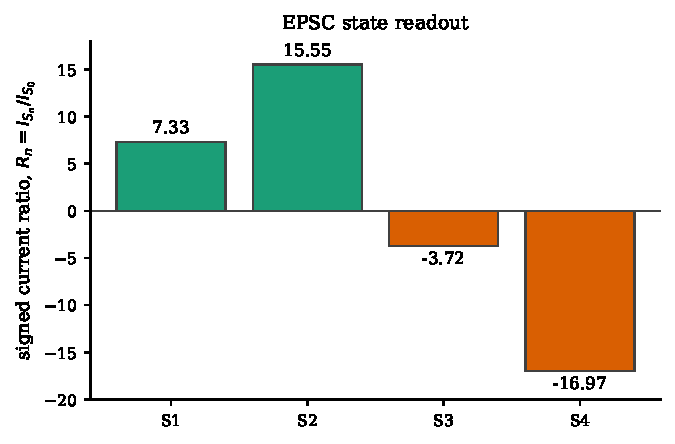
\includegraphics[width=\linewidth]{../figures/chapter2/epsc_summary.pdf}
    \caption{EPSC state ratios.}
    \label{fig:epsc}
  \end{subfigure}\hfill
  \begin{subfigure}[t]{0.48\linewidth}
    \centering
    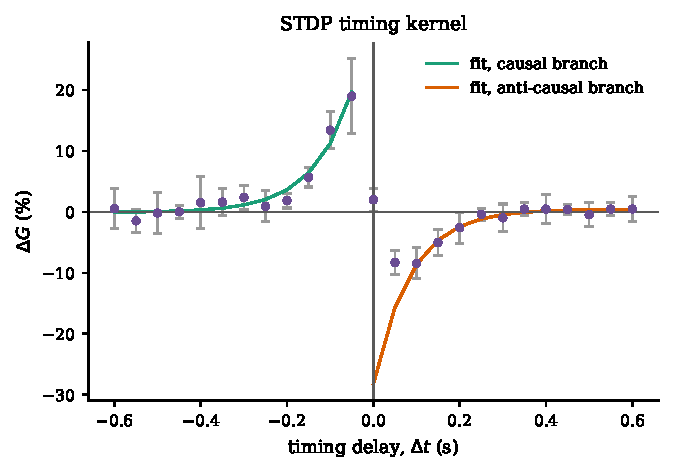
\includegraphics[width=\linewidth]{../figures/chapter2/stdp_summary.pdf}
    \caption{STDP timing kernel.}
    \label{fig:stdp}
  \end{subfigure}
  \caption[Compact EPSC and STDP summary]{Compact summary of the extended synaptic measurements. \textbf{(a)} Signed EPSC readout ratios \(R_n=I_{S_n}/I_{S_0}\) for the four demonstrated states. \textbf{(b)} Spike-timing dependent plasticity: percentage conductance change \(\Delta G\) as a function of the pre/post spike-timing delay \(\Delta t\), with each branch fitted to the decaying exponential of \cref{eq:stdp_fit}. Data and reported state ratios from Ref.~\cite{PradoSocorro2022}; STDP curve regenerated from the local NM\_v055 Day19 archive.}
  \label{fig:extended_synapse_summary}
\end{figure}

The result that the obtained learning rule corresponds to \textit{asymmetric Hebbian} STDP reflects the specific voltage waveform design, the stated definition of \(\Delta t\), and the polarity conventions of the electrode configuration. Different waveform designs or an opposite sign convention would be expected to produce differently labelled STDP kernels, offering an additional degree of tunability in the design of hardware neural network architectures built from these devices.


%% ------------------------------------------------------------
\section{Theoretical Framework: Ion Transport and the Origin of Memristance}\label{sec:mechanism}
%% ------------------------------------------------------------

The injection and bulk-transport physics of the composite are described by two limiting-case models inherited from the polymer light-emitting electrochemical cell (LEC) literature: an \emph{electrodynamic} (injection-limited) model~\cite{deMello1998,deMello2002} and an \emph{electrochemical-doping} (ohmic) model~\cite{Pei1995,Smith1997,Matyba2009}, which van~Reenen \textit{et al.}~\cite{vanReenen2010} reconciled as two regimes of the same field-driven ion redistribution. The equilibrium ion distribution, the thermionic-injection description, and the two models in full are set out in \chTwoSIRef{app:ch2_ion_models}; the focus here is on what they imply for the two observed memory regimes.

For the present SY/Hybrane/LiOTf system, the \SY{} polymer has moderate hole mobility and a moderate injection barrier from ITO, so both mechanisms may contribute simultaneously. The interpretation adopted here associates the ED mechanism with the rapid conductance changes at short timescales (milliseconds to seconds), driven primarily by the fast-moving triflate anions, and the ECD mechanism with the larger, slower changes at longer timescales (seconds to tens of seconds), driven by the slower-moving \ce{Li+} cations; on this reading the hierarchy of timescales is the physical origin of the STM/LTM dichotomy. It should be stressed that the device-level measurements of \cref{sec:elec_char} do not by themselves uniquely separate the two contributions: a clean discrimination would require, for instance, their temperature, film-thickness, or sweep-rate dependence, which is not pursued here. The assignment is therefore a working interpretation rather than an established fact. Its central falsifiable consequence --- that the slow timescale should track the cation--host coordination strength --- is examined directly in \Cref{ch:comparative} by varying the cation at fixed host chemistry.

\subsection{Lewis Acid-Base Chemistry and the Two Memory Regimes}\label{subsec:lewis}

The chemical mechanism proposed here for the two memory regimes is the same hard--soft acid--base reasoning developed in \cref{subsec:ion_conducting_polymers,subsec:composite_rationale}, applied to the specific salt and host of this device.

Within the HSAB framework, the strength of the interaction between a Lewis acid and a Lewis base in a coordination environment is set by the matching of their hardness or softness~\cite{Pearson1963}. The hard--hard interaction between \ce{Li+} (a small, hard Lewis acid with charge density \(z/r \approx\) \SIrange{1.3}{1.7}{\per\angstrom}) and the ether oxygen atoms of \Hybrane{} (hard Lewis bases) is governed predominantly by electrostatic forces, and is therefore thermodynamically strong and geometrically specific. In polyether environments \ce{Li+} is coordinated by four to six oxygen donors --- five in the crystalline complex \(\mathrm{PEO_3{:}LiCF_3SO_3}\) (three ether oxygens and two triflate oxygens) --- with oxygen--lithium distances of \SIrange{1.9}{2.1}{\angstrom}~\cite{Lightfoot1993}. This local site \emph{binding} should not be confused with the \emph{migration} activation barrier that governs hopping: the latter is the saddle-point barrier between adjacent sites --- of order \SI{50}{\kilo\joule\per\mol} ($\approx 20\,k_{\mathrm{B}}T$; \cref{subsec:hybrane}) --- and is therefore smaller than the full coordination well, while still being substantially larger than \(k_{\mathrm{B}}T\).

The interaction between the \ce{CF3SO3-} triflate anion and the host oxygens is, by contrast, much weaker. The diffuse, low-charge-density triflate anion does not engage in strong electrostatic interactions with the hard-base oxygen atoms, and the residual interaction is governed mainly by weak van der Waals forces~\cite{BruceVincent1993,Frech1999PEOLiTf}. The energy barrier for displacement of a triflate anion from one interstitial site to the next is therefore expected to be substantially lower than the barrier for a \ce{Li+} cation.

This differential activation barrier translates directly into a differential ionic mobility under an applied field, and hence into different voltage thresholds for significant ionic redistribution:

\begin{itemize}
  \item A modest voltage of \SI{1}{\volt} applied across a \SI{209}{\nano\metre} film generates a field of approximately \SI{4.8}{\mega\volt\per\metre}. In the interpretation adopted here, this is sufficient to drive the more weakly bound triflate-anion redistribution observed experimentally~\cite{PradoSocorro2022}. The fast anionic redistribution produces a rapid conductance change, which then relaxes on the timescale of triflate diffusion through the host. This is the \STM{} regime, with retention \SIrange{10}{15}{\second}, driven primarily by triflate relaxation.

  \item A voltage of \SI{3}{\volt} across the same film generates approximately \SI{14.4}{\mega\volt\per\metre}. This higher field is assigned to the onset of a slower cation contribution, consistent with the stronger \ce{Li+} coordination expected in oxygen-rich polyether hosts~\cite{Lightfoot1993,BruceVincent1993}. The cation contribution sets in, produces a delayed and stronger ionic redistribution, and relaxes on the much longer timescale of cation re-coordination. This is the \LTM{} regime, with retention exceeding \SI{45}{\second}, driven primarily by cation redistribution.
\end{itemize}

This account yields a specific, experimentally testable prediction. Replacing \ce{Li+} with a monovalent cation of larger ionic radius (\ce{Na+} or \ce{K+}) should reduce the charge density, and therefore the hardness, of the Lewis acid. The cation--oxygen coordination with the polyether host should weaken accordingly, and the slow fading-memory timescale of the device should shorten as the cation is moved along the \ce{Li+} \(\to\) \ce{Na+} \(\to\) \ce{K+} series. The prediction is tested in \Cref{ch:comparative} on the main comparative corpus of the thesis: a PEO-based polymer-electrolyte series loaded with lithium, sodium and potassium triflate salts (PEO/LiOTf, PEO/NaOTf, PEO/KOTf) at fixed polymer and salt mass fractions, complemented by a dedicated PEO/LiOTf concentration sub-study. The prediction is addressed there as a statement about the shift of the measured variable-delay depotentiation timescale when the cation is varied at fixed host chemistry, not as a claim about the full synaptic suite reported in the present chapter.


%% ------------------------------------------------------------
\section{Device Stability and Reproducibility}\label{sec:stability}
%% ------------------------------------------------------------

\subsection{Ambient Shelf Stability}\label{subsec:lifetime}

Two distinct notions of device longevity must be kept separate. \emph{Cycling endurance} --- the number of write/erase cycles a device sustains before its performance parameters drift outside specified tolerances --- is the metric that ultimately governs suitability for the millions-to-billions of weight updates of on-chip training; it is not characterised for the present devices and is left for future work. \emph{Shelf (calendar) stability} --- the retention of performance during storage and intermittent operation under ambient conditions --- is what is reported here. It is the more immediately relevant metric at the proof-of-concept stage, where the question is simply whether the unencapsulated composite survives realistic handling at all.

The devices reported here were characterised at regular intervals over a period of two weeks (\SI{{\sim}300}{\hour}) after fabrication, without encapsulation, while stored in ambient air at room temperature. The key metrics monitored were the baseline conductance $G_0$, the maximum achievable conductance change $\Delta G_{\mathrm{max}}$, and the STM retention time $\tau_S$; the supporting stability record is collected in \chTwoSIRef{app:ch2_morphology_stability}.

The results show that all three metrics remain within \SI{20}{\percent} of their initial values over the full two-week measurement period~\cite{PradoSocorro2022}. This stability compares favourably with other organic memristive devices reported in the literature, which typically exhibit significant degradation within hours to days under ambient conditions~\cite{Shih2016}. The enhanced stability is attributed to the solid-state nature of the composite: unlike devices based on liquid electrolytes or gel polymers, the Hybrane matrix provides a mechanically cohesive environment that protects the ions from evaporation and the polymer films from delamination, consistent with the stability of related Hybrane-based LEC blends~\cite{Mardegan2021}.

\subsection{Device-to-Device Reproducibility}\label{subsec:reproducibility}

Reproducibility is a persistent challenge for memristive devices, particularly those based on filamentary switching in inorganic materials, where the stochastic nucleation of conducting filaments produces large device-to-device and cycle-to-cycle variability~\cite{Sun2019}. The present system, which operates by uniform bulk ionic redistribution rather than localised filament formation, is intrinsically less susceptible to this type of variability.

The strongest reproducibility statement available from the archived proof-of-concept data is the one attached to the pulse-number experiment in \cref{fig:npulse}. That dataset contains five independent crossbar pixels on the NM\_v055 substrate, measured under the same \SI{1}{\volt} write and \SI{150}{\milli\second} wait protocol. The shaded band is one standard deviation across those five pixels. For $N_{\mathrm{pulses}} < 100$, the median RSD is \SI{8.9}{\percent} and the largest RSD is \SI{11.8}{\percent}; the appropriate claim is therefore reproducibility at about the \SI{10}{\percent} level in the low-pulse-count regime, not an exact upper bound below \SI{10}{\percent}.

The EPSC readout and STDP measurements remain important protocol demonstrations, but the recovered archive does not contain a normalized EPSC population table comparable to the PULSES and DELAYTIME tables used later in the thesis. They are therefore not used to support an independent EPSC RSD claim here. Likewise, the published proof-of-concept data establish same-substrate/pixel reproducibility and two-week shelf stability; they should not be read as a powered batch-to-batch reproducibility study. Campaign-scale reproducibility --- a separate metric on a separate axis --- and its resolution by a change of ion-transport host are taken up in \cref{ch:bridge}.


%% ------------------------------------------------------------
\section{Comparison at the Time of Publication}\label{sec:comparison}
%% ------------------------------------------------------------

The historical comparison table reproduced in \chTwoSIRef{tab:ch2_historical_comparison} places this device alongside representative organic and hybrid memristive devices available at the time of the 2022 publication. Two combinations stand out as unrepresented in that set. The first is the coexistence of \STM{} and \LTM{} in a single \emph{fully reversible} 2-T device: the closest prior report, Liu \textit{et al.}~\cite{Liu2016}, achieved short-to-long-term transitions but through irreversible redox chemistry~\cite{Heremans2011}, whereas here the conductance returns to \(G_0\) after the reset protocol. The second is STDP in a 2-T architecture, where the timing rule emerges from the superposition of pre- and postsynaptic pulses at the single Ag terminal rather than from the gate of a 3-T device~\cite{Gkoupidenis2015,Kim2018,Seo2019}. On the operating-regime axes the device is competitive in unencapsulated shelf lifetime (\(\sim\)\SI{300}{\hour}, roughly an order of magnitude beyond comparable organic devices~\cite{Shih2016}) but not in energy per event (\(\sim\)\SI{50}{\nano\joule}, above CMOS and inorganic-memristor budgets~\cite{IndiveriLiu2015,YangStrukovStewart2013}); the full table and a per-axis discussion are given in \chTwoSIRef{app:ch2_comparison}.

The comparison above retains the device-level metrics conventional in the organic memristive literature of the early 2020s: reversibility, retention window, energy per event, and operational lifetime. Subsequent work has broadened the field substantially, particularly through organic electrochemical neurons and neuromorphic circuits~\cite{Harikesh2024OECNReview,Krauhausen2024Robotics} and through the wider organic-iontronic memristor landscape~\cite{Xia2024OIMReview}. The table is therefore used only to locate the 2022 proof-of-concept result historically. Within the thesis-wide argument, those metrics play a narrower role: they establish that the polymer-electrolyte platform introduced here is reversible, dynamically addressable, and stable enough to support the comparative study of \Cref{ch:comparative} (a PEO-based triflate composition and cation sweep, characterised through the same three common dynamical measurements) and the temporal-computing reinterpretation of \Cref{ch:temporal} built on those measurements. They are not invoked to claim that this device should be judged by the standards of a high-density non-volatile memory technology, nor to suggest that the full synaptic suite reported here is available across the full comparative corpus. Those measurements remain specific to the present SY/Hybrane/LiOTf device.


%% ------------------------------------------------------------
\section{Summary}\label{sec:ch2_summary}
%% ------------------------------------------------------------

This chapter has reported the design, fabrication, and characterisation of a fully reversible 2-T organic memristive device that supports, within a single polymer-composite active layer, a full set of synaptic functions organised in two families: the three dynamical measurements carried through the rest of the thesis (I--V hysteresis, variable-number-of-pulses potentiation, and variable-delay depotentiation), and the extended synaptic protocols specific to this device (EPSC, the separated \STM{}/\LTM{} reading of the retention data, and \STDP{}).

A ternary \SY{}/\Hybrane{}/\LiTf{} composite satisfies the three functional requirements of \cref{subsec:design_rationale} (electronic pathway, ion-transport medium, ion source), fabricated as a 2-T ITO/composite/Ag sandwich by solution processing and one evaporation step, with a \SI{209}{\nano\metre} active layer below \SI{3}{\nano\metre} RMS roughness. On this single platform the three dynamical measurements carried forward to the comparative corpus were established: analogue I--V hysteresis (a \SI{140}{\percent} conductance rise from cycle~1 to~2 at \SI{1}{\volt}); fully reversible pulse potentiation/depression exceeding \SI{200}{\percent} at \(\sim\)\SI{50}{\nano\joule} per event, growing past \(10^3\%\) for \(N_{\mathrm{pulses}}>10^3\); and variable-delay depotentiation resolving two regimes (\STM{}, \(\tau_S=\SIrange{2.57}{3.01}{\second}\), retention \SIrange{10}{15}{\second}; \LTM{}, \(\tau_L=\SI{4.73}{\second}\), retention \(>\SI{45}{\second}\), from $\beta=1$ fits). The extended single-device protocols add a four-state EPSC read-out (signed ratios \(-17\) to \(+16\)) and an asymmetric-Hebbian STDP window (\(\tau=\SIrange{85}{90}{\milli\second}\), biologically realistic~\cite{Bi1998,Kuzum2013}). The \STM{}/\LTM{} dichotomy is attributed to the Lewis acid--base mobility asymmetry between the weakly coordinated triflate anion and the strongly coordinated \ce{Li+} cation in the oxygen-rich host, with the injection and bulk-transport physics described by the electrodynamic and electrochemical-doping models in their reconciled form~\cite{vanReenen2010} (\chTwoSIRef{app:ch2_ion_models}). Devices were stable over a \(\sim\)\SI{300}{\hour} unencapsulated ambient shelf (cycling endurance not characterised), with \(\sim\)\SI{10}{\percent} low-pulse-count variability across five pixels on NM\_v055 (median RSD \SI{8.9}{\percent}); campaign-scale reproducibility is taken up in \cref{ch:bridge}.

Taken together, these results establish the SY/Hybrane/LiOTf composite as a thoroughly characterised exemplar of a polymer-electrolyte organic memristive device, and identify cation--polyether coordination chemistry as the physical hypothesis for memory-timescale control. This identification motivates the main comparative study of \Cref{ch:comparative}, which replaces \Hybrane{} with poly(ethylene oxide), varies the PEO/LiOTf composition as the replicated quantitative axis, and surveys host, anion, and cation substitutions as sample-limited chemical side evidence. In \Cref{ch:comparative}, the hypothesis is tested through the three common dynamical measurements (I--V hysteresis, variable-number-of-pulses potentiation, and variable-delay depotentiation) that are abundant across the comparative corpus; the outcome is deliberately cautious, with no robust host- and anion-independent Li/Na/K law claimed. The richer synaptic metrics reported in the present chapter (EPSC, separated \STM{}/\LTM{} retention, and STDP) are not propagated to the later chapters and serve there only as lithium-device priors and sanity checks. Beyond this comparative handoff, the volatile two-timescale behaviour established here is the experimental anchor for the temporal-computing reinterpretation of \Cref{ch:temporal}, in which behavioural models fitted to the \Cref{ch:comparative} corpus drive reservoir-computing simulations, physiological temporal-context reconstruction, and WESAD affective-computing demonstrations. In those paradigms, the fading memory of the device is the active computational resource rather than a retention defect to be suppressed.


%% ---- Standalone close (skipped when \include'd from thesis.tex) ----
%% A unified bibliography is printed from thesis.tex in the thesis build,
%% so the per-chapter \printbibliography runs only in standalone mode.
\ifdefined\thesismode
  \let\thesisstandaloneclose\relax
\else
  \printbibliography[heading=bibintoc, title={References}]
  \def\thesisstandaloneclose{\end{document}}
\fi
\thesisstandaloneclose
